\section{Implementation}
\label{s:implement}

\subsection{MATLAB Implementation}
\label{s:implement_matlab}

\paragraph{}
The algorithms as mentioned in Section 3.5 require computations 
of large matrices. In particular, they require eigenvalue computations, 
matrix-matrix multiplications, matrix-vector multiplications and other 
algebraic transformations. Considering MATLAB's capabilities to perform 
the required computations with programming abstractions, it is considered 
as an appropriate tool for initial implementations. Also, MATLAB's Toolbox 
for Image Processing provides additional advantage for exploratory analysis 
of images from Radio Interferometry data sets. 

\paragraph{}
Further, algorithmic implementations were developed for all four variants 
of Iterative Shrinkage Thresholding Algorithms. Exploratory analysis via 
empirical validation were carried out by investigating the run-time complexities 
of the algorithms. CPU time taken were recorded, compared and evaluated. 
Performance benchmark trials were carried out by varying the number 
of iterations and the penalty parameter for determining their optimal values. 
Objective function values at each iteration were stored with a specified
numerical accuracy. Robustness of the algorithmic implementation was validated
by performing repeated trials with varying data sets each representing 
single point source, double point sources and grid point sources.

\subsubsection{Input Data}

\paragraph{}
Initially, data sets with characteristics similar to the original data sets
of the FITS files were simulated using the AIPS tool for single point source 
and double point sources with varying fluxes. Each row of data set consist of
a $u,v,w$ co-ordinates, amplitude and phase of visibility measured. 

\subsubsection{Processing}

\paragraph{}Parameters required for processing the data sets are
\begin{itemize}
 \item Lipschitz constant ($L$) for fixed step size variants which is maximum
	eigenvalue of $A^\dagger A$.
 \item Backtracking parameter ($\eta$). For both backtracking variants $\eta$ value
       is taken as 1.125.
 \item Penalty parameter ($0 < \lambda < \infty$).
 \item Maximum Iteration Number ($maxiter$) which is one of the stopping criterion formats 
	the algorithms.
 \item Tolerance limit explained by equation (\ref{stopping}).
\end{itemize}

\paragraph{}
After parameters are decided, $A$ matrix is computed using $u-v$ co-ordinates from data sets
and regular $l-m$ grid using equation (\ref{Amat}). Visibilities are computed in $a+ib$ format
using phase and amplitude and were stored in $b$ vector which is our measurement vector.  
Further, each variants of algorithms require $A^ \dagger A$, $A^ \dagger b$ 
which are computed as discussed in Section 3.7. Finally, following processed inputs are
given to algorithms
\begin{itemize}
 \item $A^\dagger A$
 \item $A^\dagger b$
 \item Lipschitz constant ($L$) (for fixed step size)
 \item Penalty parameter ($\lambda$) 
 \item Backtracking Parameter ($\eta$) (for backtracking)
 \item Initial guess of solution which is zero vector
 \item Maximum iteration ($maxiter$)
 \item Tolerance limit (typically $10^{-7}$) 
\end{itemize}

\subsubsection{Output data}
\paragraph{}All four algorithms gives exactly the same solution vector with high numerical
accuracy for single point source and double point source data set. By plotting the objective 
function values with each iterations it was clear that FISTA variants perform better than 
ISTA. Further, backtracking algorithms scores over fixed step size algorithms for radio interferometric
data sets.

\subsection{C Implementation}
\label{s:implement_C}

\paragraph{}For the reasons of speed, efficiency, flexibility and to include 
Compressed Sensing formulation in GMRT pipeline, all algorithms are implemented in C.
Radio Interferometry data sets are available in Flexible Image Transport System 
(FITS) formats (see appendix). We use Read-Write FITS (RWFITS) \footnote{written by Prof.\ Jayaram N. Chengalur}.
for reading the FITS file, in a specific structure which is further read for 
$u,v,w$ and visibility data.

\paragraph{}The structure of C-code is shown in Figure (\ref{Figflow}). The Data, after being read 
from FITS file are given to processing block which compute the inputs needed by algorithms 
as discussed in previous section. Since there is lot of symmetry in $A^ \dagger A$ (discussed in Section 3.7)
 and $A$ (due to symmetry in $uv$ plane), there are options in the code for using these symmetries.
Finally these computed matrices are given to the Compressed Sensing solvers, each algorithm gives same solution image
with high precision accuracy. This reconstructed solution image is written back in to FITS file format using
cfitsio (see appendix) routines.

\paragraph{}For Basic linear algebra operations we have used intel's implementation of LAPACK and BLAS library,
which performs matrix-matrix, matrix-vector, eigenvalue computations efficiency.

\begin{figure}[!htbp]
  \begin{center}
      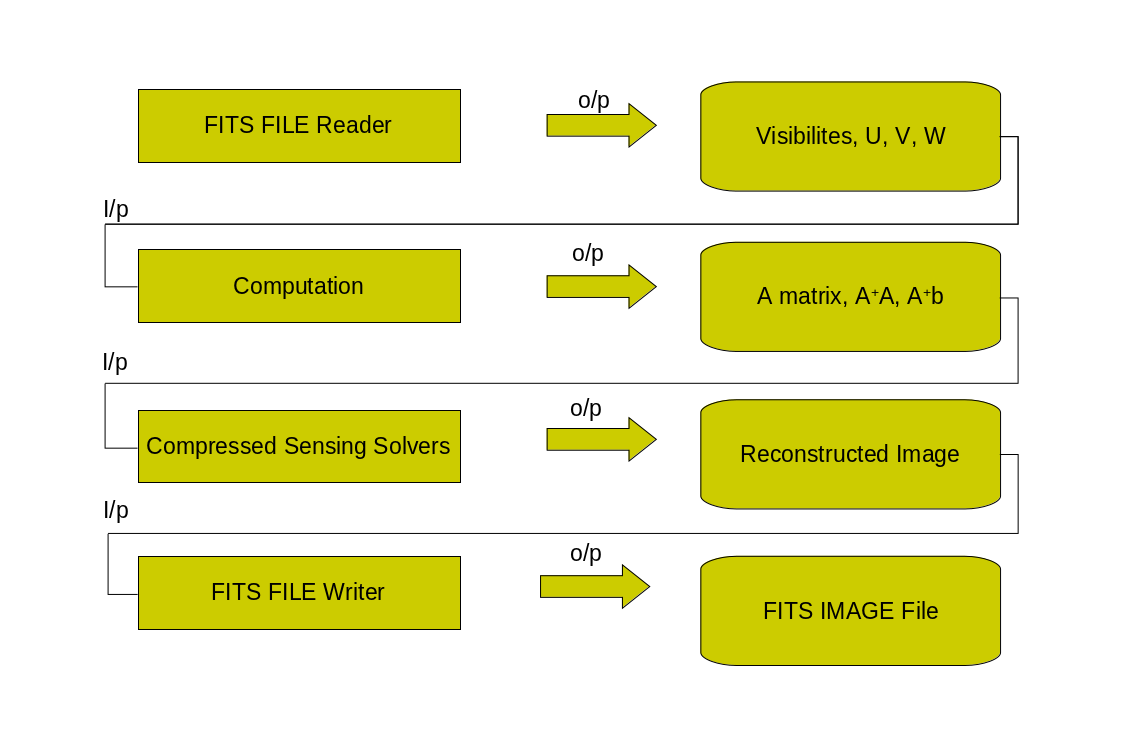
\includegraphics[width=6.1in,height=4in]{figures/flow}
    \caption{Flowchart of C Code}
    \label{Figflow}
  \end{center}
\end{figure}
